\chapter{时间-空间网络中多条最短路算法设计}\label{ch:时间-空间网络中多条最短路算法设计}
多条最短路有两个核心特点: 一个是多,一个最短。首先,最短路算法是智能交通系统的核心。
在构建城市智能交通系统中,最重要的就是选择最优的路径规划算法,实现在复杂的城市路网中找出最适合用户的路径其次,最短也有多层含义,根据不同驾驶者的需求差异,或要求距离最短,或要求时间最短,或要求可靠性高。
同时,在具体的出行方式中可能还有各种细分的出行需求,例如在选择地铁出行方式中,可能还有换乘最少等需求;
在选择公交出行方式中,可能有步行最少等需求。
此外,即使是同一驾驶者,在不同的时间节点的出行需求很大可能是不同的,
例如在上班途中,一般来说都是尽可能选择最短时间,最短距离的路径从而快速到达公司,避免迟到。
而在下班途中,即使绕道,可能也需要去某些大型连锁超市购买晚餐的食材。
多条最短路可以避免因网络中路段的故障,例如路段施工维护等原因造成目的地不可达,提高了路径选择算法的容错性和ITS的可靠性。
综上所述,多条最短路一能提供最为经济或效率最高的出行方式。
二能根据用户的差异性需求提供个性化的路径导航。
三能提高系统的可靠性。
所以说,多条最短路问题的研究对人们的日常生活用着极大的影响。

时间-空间交通网络属于动态网络,而动态网络中的最短路径的求解依赖于静态网络中最短路的基础,而k条最短路问题属于最短路径问题的变体。
因此接下来我们将首先研究静态网络中的最短路算法设计,再研究静态网络中的k条最短路算法的设计,
最后根据第三章对时间-空间网络模型的表示方法,将时间-空间网络中k条最短路问题转化为一个时间拓展图中的k条最短路问题,从而实现对动态网络中k条最短路算法的设计。


\section{单源最短路算法设计}\label{sec:单源最短路算法设计}
有很多算法在图形上运行。本文将主要介绍广度优先搜索,Dijkstra算法和A-star算法。

广度优先搜索在所有方向上都进行了同等的探索。这是一个非常有用的算法,不仅适用于常规路径查找,还适用于程序地图生成、流场路径查找、距离地图和其他类型的地图分析。

Dijkstra的算法(也称为统一成本搜索)让我们可以优先选择要探索的路径。与其平等地探索所有可能的路径,它更倾向于低成本的路径。我们可以分配更低的成本来鼓励在道路上移动,更高的成本来避免形成搜索森林,更高的成本来阻止接近敌人,等等。当移动成本发生变化时,我们使用这种方法,而不是广度优先搜索。

A-star是对Dijkstra算法的修改,该算法针对单个目的地进行了优化。Dijkstra算法可以找到所有位置的路径;A-star查找到一个位置或几个位置中最近位置的路径。它优先考虑那些似乎更接近目标的路径。

\subsection*{Dijkstra算法}
Dijkstra算法首先将全部节点集合分为两个集合:S集合和T集合。其中S集合表示已确定最短路径长度的节点的集合,而T集合表示未确定最短路径长度的节点的集合。
算法初始化时网络中的所有结点均属于T集合,首先将除源点s外其它所有点的距离初始值为无穷大,不断重复执行从T集合中取出到源点s具有最短路径的结点q,将其加入到集合S中,并对结点q的出边执行松弛操作直至集合S中包含网络中的全部节点


\begin{algorithm}
    \caption{Dijkstra算法}
    \begin{algorithmic}[1]
        \STATE 初始化: $S = \{s\}, T = U - S, dis(s)=0, dis(u)=+\infty$
        \REPEAT
        \STATE 取$q=\min(dis(u)), u \in T$
        \STATE $T.pop(u), S.push(u)$
        \STATE relax(u)
        \UNTIL S.length == N
        \STATE 算法结束
    \end{algorithmic}\label{alg:algorithm}
\end{algorithm}

\subsection*{A-star算法}
在导航系统中,我们经常需要找到从一个位置到另一个位置的可行路径,在更好的情况下,我们努力寻找系统中的最短路径,可能需要考虑到旅行时间,距离等。
为了找到这条路径,我们可以使用图形搜索算法A-star算法,A-star算法作为一种启发式算法,是图形搜索算法的常用选择。一般情况下,A-star算法以Dijkstra算法作为基础来寻找估计距离,
Dijkstra算法可以很好地找到最短的路径,但它会浪费时间去探索那些没有可能是最短路的方向。贪婪的“最佳优先搜索”(Best First Search)朝着有希望的方向探索,但它可能找不到最短的路径。
A-star算法使用从开始的实际距离和估计到目标的距离,即f(n)=g(n)+h(n),其中f(n)表示总成本,g(n)表示从开始位置到当前位置已经花费的成本,而h(n)表示从当前位置到目标位置的预计成本。

A-star算法首先需要定义open表和close表,在open表中存放已知但还未访问过的节点,在close表中存放已经访问过的节点;
再定义估价函数或启发式函数h(n),用来度量剩余距离,一般使用Dijkstra算法进行计算;
算法初始化时把起始节点加入到open表中,重复执行下面的操作
\begin{enumerate}%有序列表
    \item 如果open表为空,则寻路失败,找不到达到终点的路径。
    \item 遍历open表,选择总成本最小的节点作为接下来要处理的节点,并把这个节点加入到close表中
    \item 处理该节点的所有邻接节点
    \begin{enumerate}%有序列表
        \item 如果邻接节点在close表中,表示邻接节点在之前已经访问过,忽略即可;
        \item 如果邻接节点不在open表中,则把邻接节点加入到open表中,并将当前节点设置为邻接节点的父节点,计算邻接节点的总成本
    \end{enumerate}
    \item 如果终点加入到open表中,此时说明已经找到最佳路径,而由起点到终点以及之前关联的父节点便构成了一条最优路径
\end{enumerate}

\begin{algorithm}
    \caption{A-star算法}
    \begin{algorithmic}[1]
        \STATE 初始化: open =$\{s\}$, close
        \STATE 定义启发式函数h(n)
        \STATE 计算估计距离f(n) = g(n) + h(n)
        \STATE open.length == 0, 不存在最短路, 算法结束
        \REPEAT
        \STATE 遍历open表, 选择f(n)最小的结点u
        \STATE open.pop(u), close.push(u)
        \STATE 寻找u的邻接节点v
        \STATE  open.push(v),
        \STATE  计算结点v的估计距离
        \UNTIL open.length == 0
        \STATE 算法结束
    \end{algorithmic}\label{alg:algorithm2}
\end{algorithm}


\section{多条最短路算法设计}\label{sec:多条最短路算法设计}
首先借助下面的简单路网说明以下偏离点和偏离路径的概念,
在图\ref{fig:fig12}中可以通过上面介绍的经典的单源最短路算法,
如Dijkstra算法或A*算法求得源点s到汇点t的最短路径p1为$s\to 1\to t$,
路径成本代价为1+3=4。
在k最短路径中,除汇点t之外路径上的其它节点,
都被称为偏离点。而源点s到汇点t的次短路径p2为$s\to 1\to 2\to t$,路径成本为1+2+2=5,
此时路径p2相对于路径p1的偏离节点为节点1,即节点1为路径p1到路径p2的偏离点,
而路段$1\to 2\to t$被称为路径p1到路径p2的偏离路径。
\begin{figure}[H] %H为当前位置,!htb为忽略美学标准,htbp为浮动图形
    \centering %图片居中
    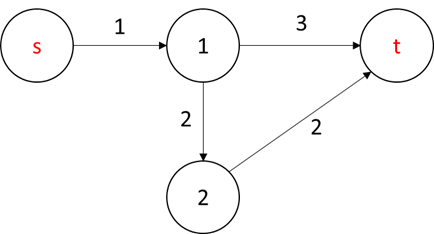
\includegraphics[width=0.7\textwidth]{png/图片12偏离点和偏离路径} %插入图片,[]中设置图片大小,{}中是图片文件名
    \caption{偏离点和偏离路径} %最终文档中希望显示的图片标题
    \label{fig:fig12} %用于文内引用的标签
\end{figure}

\subsection{设计思路}\label{subsec:设计思路}
该算法可以分为两个步骤,首先确定第一条最短的路径,即$A^1$,然后依次确定其他k-1条次短路径。
假定使用容器A来保存最短路径,而容器B将保存可能的k最短路径。
为了确定从起点到终点的k条最短路径,可以使用有效且高效的单源最短路径算法。

为了找到第k条最短路$A^k$,k的范围从2到K,
算法假设在寻找第k条最短路$A^k$之前已经发现了从$A^1$到$A^(k-1)$的所有路径。
因此第k轮迭代可以分为两个阶段:(a).找到所有的$A_i^k$;
(b).从所有的$A_i^k$中找出最短路径即为$A^k$。
在此迭代过程中,i的范围从1到$Q_k^k$。第一个过程可以进一步细分为三个操作,
(a).选择$R_i^k$,(b).寻找$S_i^k$,(c).将$A_i^k$添加到容器B中保存作为第k最短路的候选路径。

通过在上一次寻找到的最短路径$A^{k-1}$中一次选择除汇点之外的节点j作为偏离节点$A^j$,找到从源点到偏离节点的路径作为根路径$R^k_i$。
然后在偏离点容器中查找该偏离点出边所对应的路段,如果找到路径,则将相应路段的路段阻抗$d_{i(i+1)}$设置为无穷大。
接下来,通过偏离节点到汇点的最短路径找到偏离路径。确保偏离路径和偏离路径容器中的路径不同,添加根路径和偏离路径。
接下来,删除的路段(即将其成本设置为无限)恢复为初始值。
第二个过程通过在成本最低的容器中找到路径来确定合适的路径。该路径从容器中删除并插入容器中,该算法继续进行下一轮迭代。

\subsection{算法流程(伪代码描述)}\label{subsec:算法流程}
\begin{lstlisting}[label={lst:lstlisting7}]
function KSP(Graph, source, sink, K):
    // 首先通过Dijkstra算法初始化第一条最短路径
    A[0] = Dijkstra(Graph, source, sink);
    // 准备一个存放偏离路径的容器, 最为最短路径的备选路径
    B = [];
    // 通过迭代的方式, 依次顺序地计算出从第2条到第K条最短路径
    for k from 1 to K:
        for i from 0 to size(A[k − 1]) − 2:
            spurNode = A[k-1].node(i);
            rootPath = A[k-1].nodes(0, i);
            for each path p in A:
                if rootPath == p.nodes(0, i):
                    remove p.edge(i,i + 1) from Graph;
            for each node rootPathNode in rootPath:
                remove rootPathNode from Graph;
            spurPath = Dijkstra(Graph, spurNode, sink);
            totalPath = rootPath + spurPath;
            if (totalPath not in B):
                B.append(totalPath);
            restore edges to Graph;
            restore nodes in rootPath to Graph;
        if B is empty:
            break;
        // 排序, 获取当前轮次中所有可能是最短路径的偏离路径, 选择最短的路径
        B.sort();
        A[k] = B[0];
        // 选择最短的偏离路径, 并将其从容器中弹出
        B.pop();
    return A;
\end{lstlisting}


\section{时间-空间网络下的多条最短路算法设计}\label{sec:时间-空间网络下的多条最短路算法设计}
将输入的时间聚集图转换为方便计算机处理的时间拓展图
在时间拓展图中获得k条最短路, 原问题转化为6个起始节点到6个目标节点的最短路问题
算法缺点:
在计算机实际存储过程中, 时间空间网络会成倍消耗存储空间, 假设路段离散化序列的长度为k, 则存储的节点数是原来的k倍, 存储的路段数是原来的k^2倍
不适用于大规模网络, 因此对于大规模网络可能需要使用道路网络分层的思想

\subsection{模型存储结构设计}\label{subsec:模型存储结构设计}
在静态最短路算法中,我们只需要使用一个数字即可存储路段阻抗,因此可以使用邻接矩阵或者邻接表来存储静态网络。
一般来说,邻接矩阵适合存储稠密图,即$m\approx n^2$,
邻接表更适合存储稀疏图,即$m \ll n$。
而交通网络作为典型的一种稀疏图,所以选择邻接表进行存储,
例如对于图\ref{fig:fig2}所示的静态网络采用邻接表存储结果如图\ref{fig:fig13}所示。
\begin{figure}[H] %H为当前位置,!htb为忽略美学标准,htbp为浮动图形
    \centering %图片居中
    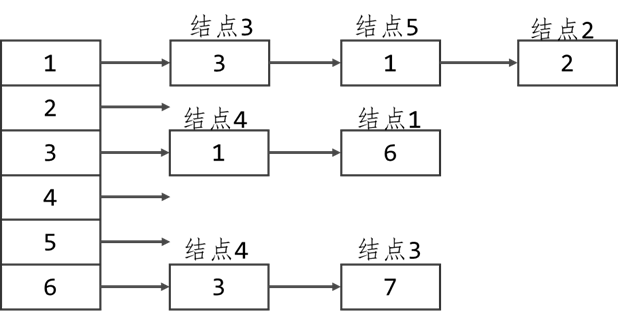
\includegraphics[width=0.7\textwidth]{png/图片13静态网络存储结构图} %插入图片,[]中设置图片大小,{}中是图片文件名
    \caption{静态网络存储结构图} %最终文档中希望显示的图片标题
    \label{fig:fig13} %用于文内引用的标签
\end{figure}

但在动态网络的最短路算法中,路段的阻抗是一个时间序列,
因此需要对上述的邻接表存储方式进行改进。之前的邻接表存储方式中,
一个结点只能存放一个值,现在需要一个结点中能够存放一个序列,
以图\ref{fig:fig6}所示的动态网络为例,对于动态交通网络的存储结构设计如图\ref{fig:fig14}所示。
\begin{figure}[H] %H为当前位置,!htb为忽略美学标准,htbp为浮动图形
    \centering %图片居中
    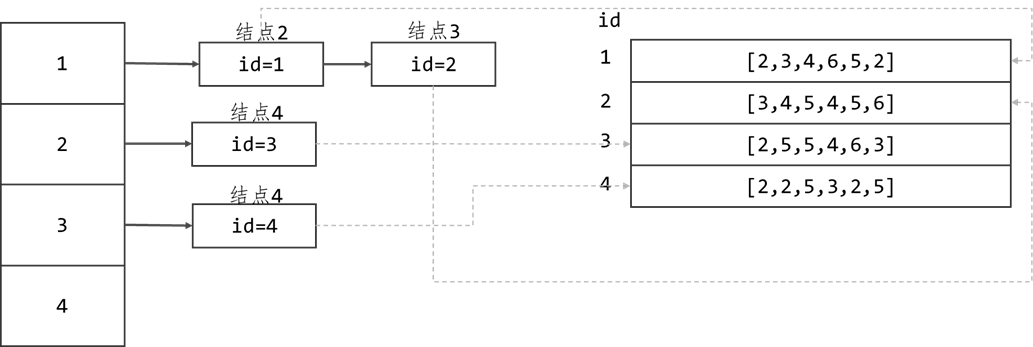
\includegraphics[width=0.7\textwidth]{png/图片14动态网络存储结构图} %插入图片,[]中设置图片大小,{}中是图片文件名
    \caption{动态网络存储结构图} %最终文档中希望显示的图片标题
    \label{fig:fig14} %用于文内引用的标签
\end{figure}

\subsection{模型求解}\label{subsec:模型求解}

\subsubsection{时间拓展图到静态网络的转化处理}
\begin{figure}[H] %H为当前位置,!htb为忽略美学标准,htbp为浮动图形
    \centering %图片居中
    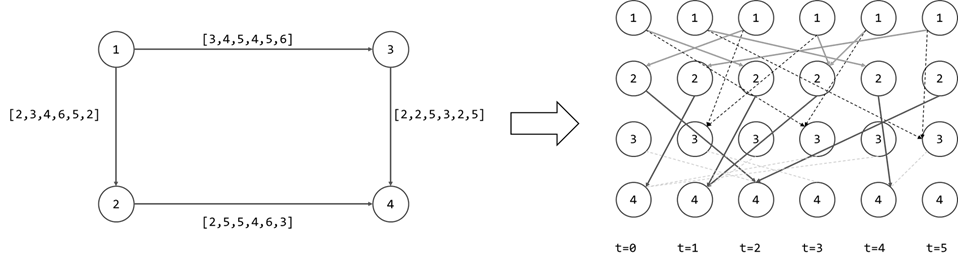
\includegraphics[width=0.7\textwidth]{png/图片15时间拓展图到静态网络的转化处理} %插入图片,[]中设置图片大小,{}中是图片文件名
    \caption{时间拓展图到静态网络的转化处理} %最终文档中希望显示的图片标题
    \label{fig:fig15} %用于文内引用的标签
\end{figure}
如图\ref{fig:fig15}所示,
根据时间拓展图中的时间序列的长度count=6,
可以将原本的时间拓展图表示为静态网络,
时间拓展图与静态网络等价的充分必要条件是满足路段阻抗和出发时刻之间的约束关系。
对于在时间拓展图中k时刻出发的任意节点from到目的节点to的约束条件
可以转化为静态网络中从出发节点(from*count + k)到目的节点(to*count+(k+cost)\%count)的一条约束,路段阻抗值保持不变。

\subsubsection{问题的等价转化}
\begin{figure}[H] %H为当前位置,!htb为忽略美学标准,htbp为浮动图形
    \centering %图片居中
    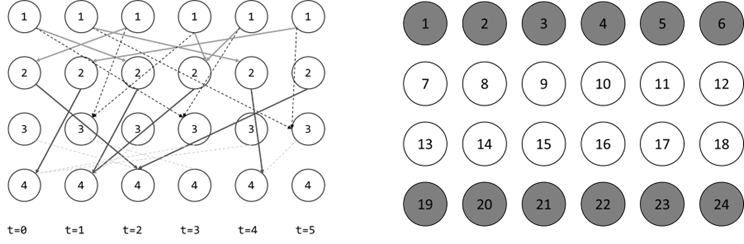
\includegraphics[width=0.7\textwidth]{png/图片16时间空间网络中k最短路问题的等价转化处理} %插入图片,[]中设置图片大小,{}中是图片文件名
    \caption{时间空间网络中k最短路问题的等价转化处理} %最终文档中希望显示的图片标题
    \label{fig:fig16} %用于文内引用的标签
\end{figure}

如图\ref{fig:fig16}所示,在时间拓展图中求解k最短路问题被等价转化为从count=6个起始节点(分别表示不同时刻出发的同一个节点)到
6个目的节点(分别表示不同到达状态的同一个节点)的最短路问题。由于实际交通网络中的路段阻抗未知,因此在
极端情况下可能存在k最短路由同一个起始节点到同一个目标节点,因此需要计算出
每一对节点之间的k条最短路径。所以原问题将被转换为6*6=36对节点之间的k最短路问题,此时需要执行36次一般物理网络下的k最短路问题。